\section{Introduction}

The new millennium saw an explosion in the development of such devices and a moving away of users from single computers towards personal computing \cite{Lyle2013}. Now, in 2017, it is commonplace for an average user to own and actively use several computing devices. With new trends and technology comes new challenges and a challenge in security arises when the user needs to manage their multiple interconnected devices and their multiple identities for their applications. The device owner usually relies on some ``Keychain'' app to share the user's cryptographic private key and this key sharing can often be insecure and expose the user to grave security concerns of theft and malware \cite{Atwater2016}. In their paper ``Why Johnny Can't Encrypt'', Whitten and Tygar \cite{Whitten} showed that major usability flaws have prevented PGP email encryption software from being widely adopted in the mainstream. A significant flaw is that users are required to interact with and manually manage their own keys. This proves too tedious of the average user and an important lesson (about why manual keychain apps are a bad idea) can be learnt from this. Devices such as phones and watches are frequently removed or replaced. Also, the loss of a single device can compromise the security of the user and their remaining devices.

In the next section, we look at the definition of this problem and look at the various possible solutions that try to solve it.

\section{Problem Statement and Solution Classes}
This section provides and overview of the multi-device problem as well as the numerous solution classes that exist. These classes all present unique approaches to solving the multi-device problem. Solutions can be implemented using just a single class or using multiple classes in combination as we shall see in subsequent sections.
In section 2.1 we talk about the multi-device problem and describe it. Section 2.2 enumerates the various possible solutions and briefly describes each one.

\subsection{The Multi-device Problem}
The multi-device problem as introduced above is a situation that arises when a user possesses several computing devices at a time. Cryptographic keys that were once simply stored on a single computer are now required by several devices and must somehow be securely distributed across these devices. Users need these to consistently authenticate themselves as the same user across multiple devices. This means that secret keys that are intended to be stored securely are now going to be moved around exposing them to multiple threats of theft such as phishing, pulling them from memory or password cracking attempts (if they are password protected) \cite{Atwater2016}.\\
The simplest solutions to this problem involve either attempting to securely synchronize a single key across multiple devices or to have a per-device key system. While these simple solutions solve the \emph{multi}-device problem, they create a set of new problems that must be addressed\cite{Atwater2016}.

\subsection{Overview of Various Solutions}
We now present an overview of the several solutions that are capable of resolving the multi-device problem as well as accompanying issues. They are as follows \cite{Atwater2016}:

\begin{itemize}

	\item \textbf{Per-device keys:} As described above, the user has an independent key on each device. The idea of per-device keys does not 				really solve the multi-device problem in that the user must generate and maintain several individual keys which is cumbersome. Also, all third 				parties must be made aware of every individual private key owned by the user to be able to consistently authenticate that user with the same 			identity. Also, unique keys for each device will keep the verifying third party informed of which device the user is currently using. This creates a 			privacy issue where third parties can monitor the usage of a user's devices just from the keys.\\

	\item \textbf{Key sync:} This involves the user making several copies of the same secret key and copying them to all devices. This procedure 				has several issues. The act of copying the secret key itself is susceptible to various attacks leading to the key being compromised. If the user 			loses one device than they must update the key for all other devices. This is because the lost device may be used to obtain the secret key and 			compromise all the other devices owned by the user.\\

	\item \textbf{Manual thresholding:} The user has per-device keys but embeds and additional police in each signature that tells the verifying 				third party to look for other signatures from other devices belonging to the user. The issue with manual thresholding is the similar to that of 				the simple per-device keys method. A verifying third party can monitor the usage of the user's devices.\\

	\item \textbf{Personal PKI:} Is one of the approaches that has seen significant interest and development. It built on the idea of the key sync 				but the user has an additional ``master'' key on one device, or a ``master'' device, or an application whose job it is to validate the other keys 			or devices. It is based on the idea of a public key infrastructure, but in this case it is entirely personal and provides the user with the 							ability to manage their own keys. The obvious disadvantage is that the user has to manage an additional ``master'' device/application and that it 	introduces a single point of failure that can be quite disastrous.\\

	\item \textbf{Group Signatures:} Group Signatures work on the idea that a single member in the group can sign a message for the other 						members. They present a single key to the third party but internally have separate keys\cite{Bellare2003}. The idea of group signatures can be 			extended to devices where the user uses one device to sign for all the other devices. This idea has been explored for the case of multiple 					password management in the form of Pico\cite{Stajano2011} where the user can use a single device to replace all their PINs and passwords. 				This has not seen significant development for the multiple devices. \\

	\item \textbf{Threshold Cryptography:} Is another approach that has seen significant interest and development. It is by far the most promising 			approach as it deals with the multi-device problem and also provides security against lost or theft of a device\cite{Desmedt2001}. In this 					method either the key itself or some cryptographic operations are distributed among the user's $n$ devices\cite{Desmedt1994}. Whenever a 			devices requires to perform a cryptographic operation, either a user defined \emph{threshold} number of devices $t$( where $t \leqslant n$) 			work together to recover the original key or the cryptographic operation itself is distributed over $t$ devices. Any less then t devices will not 			be able to divulge any valuable information.

\end{itemize}

%\mn{Add Figure from Shatter showing comparison}

%\mn{Add definitions for properties of the schemes}

\section{\emph{Personal} Key Infrastructures}

The \textit{Personal} Key Infrastructure as a solution to the multi-device problem has seen a fair share of interest over the last decade. The idea of a personal PKI has been around since the last decade. Sinclair and Smith wrote their paper during the advent of the smartphone era. It was a time when the multi-device problem was just coming into existence. To cope with it, they developed a solution in the form of \textit{porKI} \cite{Sinclair2005}.

The multi-device problem matured over the years and so did the solutions to combat it. In 2013, Lyle et al. developed and presented \textit{webinos} a cross platform runtime environment that implemented a personal PKI \cite{Lyle2013}. It directly attempts to solve the multi-device problem by extending web technologies to help users manage their devices. In 2015, Melara et al. presented CONIKS. While CONIKS does not directly address the multi-device issue, it nevertheless provides a good option to users who wish to manage their keys without having to entrust them to a third party. As such, it can be a model for solutions to the multi-device problem, and can even be used in such solutions as can be seen in the planned future work of the authors of ``Managing Identities Using Blockchains and CoSi'' \cite{Kokoris-kogias}. Essentially, the key idea behind the personal PKI is to give user's control of the their own keys and key management while at the same time making sure that they do not have to manually manage the keys and can instead remain oblivious of their existence.



%\subsection{PorKI}
%\mn{Drop old and outdated tech?}

\subsection{\emph{webinos}: Personal PKI for Smart Devices}

\textit{webinos} is an application platform designed and implemented by Lyle et al. \cite{Lyle2013}. It implements a personal network that the authors refer to as a \textit{personal zone}. These so-called personal zones define the devices that are used by a particular person. The personal zone has a master device called a personal zone hub which acts as a certificate authority and can be implemented as an online web service.

\textit{webinos} was developed in 2013 as a cross-platform runtime environment for web applications. It provides a set of JavaScript APIs for web applications to access local device functionality. For example, a web application could be made to access the camera or the address book of a smartphone. It also provides access control features to restrict and control access using the APIs for the sake of privacy and security.

Lyle et al.\cite{Lyle2013} outlined a set principles that should be adhered to while developing personal key infrastructures:
\begin{itemize}

	\item \textbf{Leverage existing identities:} Leverage the existing identities that people already have, such as social network accounts, email 				accounts and homepages, and reuse these in public key infrastructures. The authors suggest using a mapping of a social network identity to a 			public key or certificate so that users can find each other using a web-based identity.\\

	\item \textbf{Assume devices are mobile:}. Devices such as smartphones, smartwatches, tablets, laptops and cars are all designed to be 					mobile. This makes them prone to being lost or stolen. It is important that the personal PKI implementation take this into account and provide 			for such devices to be removed from the network and their keys revoked.\\
	
	\item \textbf{Avoid using PKI metaphors:} Users should not be expected to be familiar with PKI jargon and terminology. They should never be 			asked to make a decision about keys and certificates. All these should happen behind-the-scenes automatically.\\
	
	\item \textbf{Use web technologies to make networks inter-operable:} The authors suggest harnessing the power of web applications to make 			personal networks work for devices that are made to be mobile. A web server can be used to make the personal network available to any 					device that is capable of making outgoing connections.\\
	
	\item \textbf{Delegate key storage to operating systems:} The authors suggest that key storage should be delegated to the operating 						systems of the specific devices. In the authors' opinion many devices already have secure means of protecting keys such as secure hardware. 				Also, a devices like a smartphone would not have as much authentication requirements as a personal computer. Thus, the problem of key 					storage is best solved in a device-specific manner.\\
	
	\item \textbf{Device keys are not always a factor of user authentication:} The authors make room for users with shared devices. They suggest 			that device keys should be used only to authenticate the device and not the user. A device should authenticate just the device. The second 				factor (i.e. authenticating the user) is only appropriate when it is known that the device is single user specific, such as a mobile phone or a 					laptop.\\
\end{itemize}

\textit{webinos} has been designed to implement these principles. The architecture of \textit{webinos} and its implementation of a personal PKI are summarized in the following points:

\begin{enumerate}[label=\arabic*., wide, labelwidth=!, labelindent=0pt]
	\item \textbf{Components and communication:} \textit{webinos} consists of the following three components spread over various devices:
	\begin{itemize}
			\item Personal Zone Proxy (PZP) This runs on each device and implements the API. It is responsible for communicating with other PZPs, 					the PZH and Web Runtimes. It also performs policy enforcement. PZPs communicate with each other and the PZH over mutually-authenticated 				TLS 	sessions.
			\item Personal Zone Hub (PZH) The PZH is web-based and constantly available. It routes messages between PZPs and synchronizes access 				control settings. It acts as a certificate authority and issues certificates to the PZPs.
			\item Web Runtime (WRT) Web runtime is used to execute and display web applications. It is the user interface to web applications.\\
	\end{itemize}
	

	\item \textbf{Certificate hierarchy:}
		\begin{figure*}[!h]
			\centering
			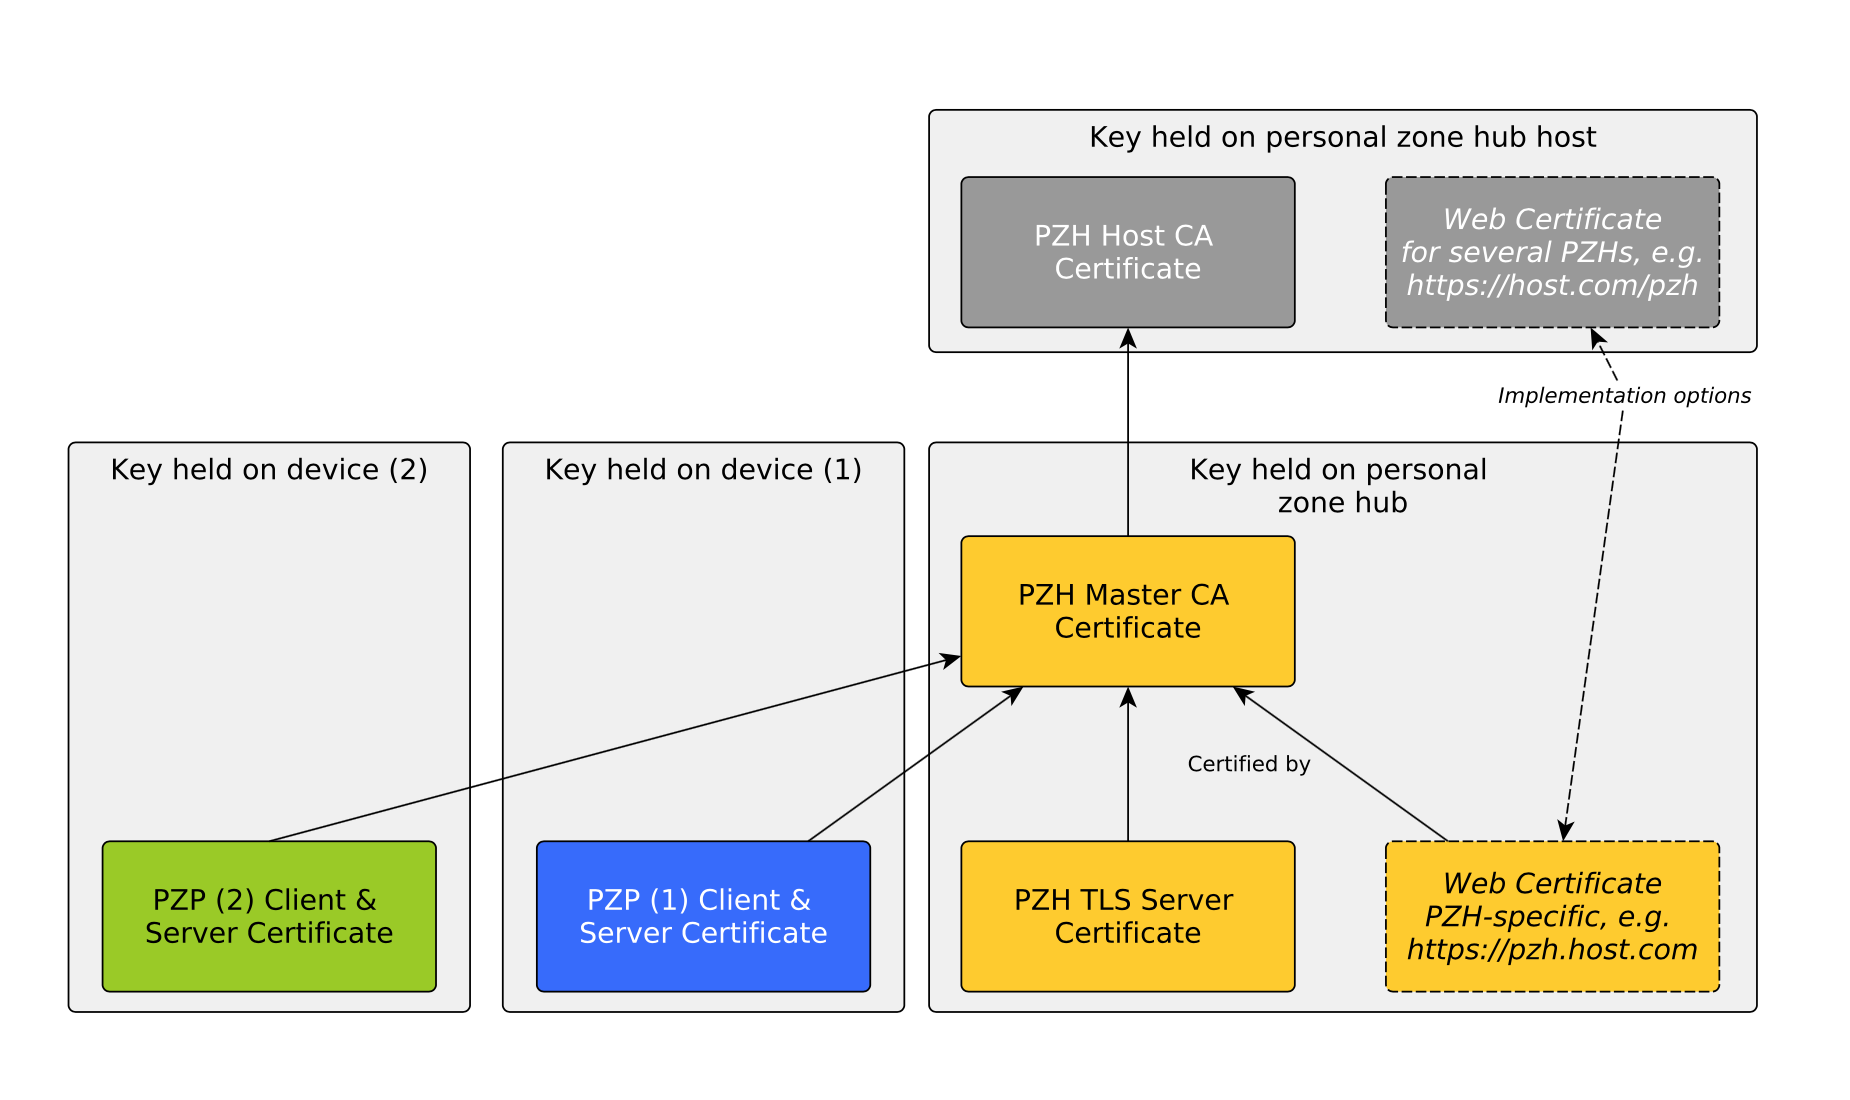
\includegraphics[width=\textwidth]{heir}
			\caption{Certificate hierarchy in \textit{webinos} \cite{Lyle2013}}
			\label{fig:heir}
		\end{figure*}
		An example of the certificate hierarchy is shown in Figure \ref{fig:heir}. The Personal zone hub acts as the certificate authority for the 					personal zones. The certificates are used to create mutually-authenticated TLS sessions. Users can host this hub on a home server if they 					wish.\\

	\item \textbf{User discovery:} An existing personal identity is linked to the \textit{webinos} personal zone hub. The authors suggest using the 			WebFinger protocol\cite{Webfinger}.\\
	
	\item \textbf{Certificate exchange:} \textit{webinos} requires that CA certificate exchange take place when two devices from different 						personal zones communicate for the first time. \textit{webinos} allows users to exchange certificates both when the devices are in close 					proximity and when they are far apart (i.e. over the internet) and has separate specifications for both. When the devices are in close 							proximity, \textit{webinos} performs a ``peer to peer offline exchange''. When a user would like to access another user's API over the 						internet, \textit{webinos} performs an ``online exchange''. For the ``online exchange'' a user (say, Alice) can visit another user's (say, Bob's) 			PZH URL and make a request to access resources. The authors have not specified what they intend to use to pair two devices in physical 					proximity for the ``peer to peer offline exchange''  plan to implement it using some word-matching or number-typing scheme. 
	
	\item \textbf{Enrolment:} Enrolment of a device has been kept relatively simple as well as user friendly. The user must install \textit{webinos} 			PZP onto their new device and then visits the PZH webpage, logs in and then simply adds a new device. The user is presented with a token such 	a 	QR code which they must enter into their new device. The specifics of the certificate exchange is completely hidden from the user.\\
	
	\item \textbf{Revocation of personal zone devices:} Similarly, revocation of a lost or stolen device is achieved quite simply by visiting the hub 				website and clicking the revoke button for that the device. \textit{webinos} deals with revocation in the following manner: Each device (PZP) is 			made to maintain a Certificate Revocation List (CRL) and must synchronize this to the hub every time it makes a new connection. The authors 			reason that this is sufficient protection against malicious attackers as it limits their window. It is worth noting at this point that \textit{webinos} 		is 	designed to protect the average user whose device would be stolen simply for the monetary value rather than an orchestrated malicious 					attack to steal the keys on it.\\
	
	\item \textbf{Access control and authentication:} When a request is made the PZP will check whether the application, device \textit{and} user 			are are authorized to make that request. \textit{webinos} does not automatically associate a device with an individual user's identity except in 			certain cases where it is known that the device is user specific. For example, a user will not have to re-authenticate every time when a policy 				request is originating from their smartphone however, they will have to re-authenticate every time if the policy request is originating form their 			TV. This is a feature, where all devices is not assumed to be user specific and share devices need users to re-authenticate, marks 								\textit{webinos} apart and makes it stand out. \\
	
	\item \textbf{Key Storage:} \textit{webinos} makes use of OS-provided mechanisms to securely store private keys. For example, the  							macOS Keychain app and the GNOME Keyring or some trusted platform-specific application. \\
	
	\item \textbf{Backup and Recovery:} The authors have decided against any form of backup or recovery for \textit{webinos}. They reason that 			the user's OpenID account (or which ever online identity is used) will already have a password recovery feature in place. Also, lost of stolen 					devices may simply be revoked. If a key is compromised on an one device, that device can simply be revoked and re-added.\\

\end{enumerate}

\subsection{CONIKS}

CONIKS is an end-user key verification service capable of integration in end-to-end encrypted communication systems\cite{Melara2015}. CONIKS eliminates the need for a third-party monitor and enables users to monitor their own keys all the while downloading less than 20 kB per day to do so. The idea behind CONIKS is that users shouldn't have to worry about manually managing encryption keys when they need to communicate securely, but at the same time they should not have to trust their communication service provider with their keys and to act in their best interest. CONIKS aims to solve this problem by using a data structure called a Merkle prefix tree which allows a single small proof (logarithmic in the total number of users) to guarantee the consistency of a user's entry in the directory. Users can monitor only their own entry without needing to rely on third parties to perform the monitoring for them.

There are four participants in CONIKS's security model:
\begin{itemize}
	\item \textbf{Identity Providers:} Identity providers run CONIKS servers.
	\item \textbf{Clients:} Users (see below) run CONIKS client software on one or more devices. CONIKS does not monitor the or address the 					problem of compromised client endpoints.
	\item \textbf{Auditors:} Monitor and audit to ensure the identity providers are not equivocating. Auditors publish and gossip with other auditors 		to ensure global consistency.
	\item \textbf{Users:} People who are using CONIKS. These users have varying needs of security and CONIKS draws a distinction between default 		users and strict users.	
\end{itemize}

CONIKS has four main protocols for operation:
\begin{itemize}

	\item \textbf{Registration and Temporary Bindings:} Is the protocol used by clients to register new name-to-key bindings or to update the user's 		public key after revocation of a key with and identity provider on behalf of the user.
	\item \textbf{Key Lookups:} Whenever a CONIKS client looks up a user's client's key to communicate with it, the identity provider also includes a 		proof of inclusion to prove the consistency of retrieved binding.
	\item \textbf{Monitoring for Spurious Keys:} CONIKS clients monitor their own bindings to check that they have not been changed.
	\item \textbf{Auditing for Non-Equivocation:} Even if a client is monitoring its own bindings, it needs to check if the identity provider is providing 		consistent versions of the keys to all participants of the system.
\end{itemize}

CONIKS provides users with the ability to choose the level of security that they want to implement. There are basically two levels at present: a default level and a strict level, both with different trade-offs between security and privacy, and usability. To present the feasibility of CONIKS, the authors have implemented a prototype called CONIKS Chat. It is a secure chat service based on the Off-the-Record Messaging plug-in for the Pidgin instant messaging client. The implementation for this prototype is no longer available on GitHub. However, the CONIKS implementation in JAVA and Go have been released and can be found on GitHub.

CONIKS is a well thought out and implemented standard upon which solutions more suited to the multi-device problem can be built. In fact, we see the authors of ``Managing Identities Using Blockchains and CoSi'' \cite{Kokoris-kogias} look to use the features of CONIKS in one of their proposed future projects.


\section{Threshold Cryptography}

The Threshold Cyptosystem approach to the multi-device problem has seen significant interest and development in the last few years. Threshold schemes were traditionally developed with organizations in mind where authority to perform actions ( such as launching missiles) is split among a number of members in a group. These members must all act together to perform the required action. This is the core idea that has been lifted and applied to the multi-device problem. It is essentially aims to turn the weakness that is owning multiple devices into a strength by using threshold schemes to distribute secrets, or perform signing and decryption operations with a combination of devices working in unison\cite{Desmedt2001, Atwater2016}. It becomes unnecessary to revoke a key if a device is stolen or lost. The user simply need to use a combination of the remaining devices to regenerate the key and create new shares among the remaining devices whilst leaving the old one out. Threshold Cryptography can also be implemented in a manner that it is invisible to the communication partner as long as threshold versions of the cryptographic algorithms used in the original app exist. The communication partner will not be aware that the user is generating signatures or performing decryption in a distributed manner.

Two examples of systems that implement thresholding are Shatter \cite{Atwater2016} and a new system for managing SSH-keys using Blockchains and Collective Signing\cite{Kokoris-kogias}. Shatter was introduced in 2016 and showcases a library called libShatter that implements threshold cryptoschemes. The second technology that uses Blockchains and CoSi was also presented as an introductory concept in 2016 and only can be used for SSH-key management. It implements a mixture of personal PKI and threshold systems and is a promising technology. The authors are currently working to provide a wider solution that can be used to manage various kinds of keys.

\subsection{Shatter}

Shatter is an open-source framework, developed and implemented by Atwater et al.\cite{Atwater2016}, that runs on desktops, Android, and Android Wear, and performs key distribution on a user's behalf. Shatter proposes to solve the multi-device problem by using Threshold Cryptography to aid in sharing a single identity across devices. Shatter aims to turn the security weakness of having multiple devices into a strength. It achieves this by using Threshold Cryptography\cite{Desmedt1994, Desmedt2001}. Apps that user Shatter can only have their keys compromised when a threshold number of devices are compromised by the same attacker. Atwater et al.\cite{Atwater2016} have developed a library called libShatter that provides implementations of threshold cryptography protocols. They have also demonstrated how Shatter can operate using two Android apps. Shatter has been used for identity key protection in the messaging app ChatSecure and for encryption key protection in the note-taking app OmniNotes.

%threat model
The authors outline three main threats to Shatter in their threat model:
\begin{itemize}
	
	\item The first case is when the user loses control of more than the threshold $t$ of their $n$ devices. This can happen due to theft, privileged 			malware running on the device and remote code execution. This is because if $x\geq t$ devices are compromised, the attacker can regenerate 			private keys. Damage mitigation and data recovery is possible when $t\leq x\leq n - t$ but not when $x>n - t$. For example, say an application is 	designed to protect a user's personal notes with threshold encryption. Both the user and the attacker have access to the notes with $t\leq x\leq 		n - t$	, however with $x > n-t$ only the adversary has access to the notes.
	\item The second threat arises when $x < t$ devices are compromised because the user has devices that automatically participate in threshold 			operations. This affords the attacker a window where they can cause harm by impersonating the user. The results of such an impersonation 				would, of course, be logged and the user may access this log later. The user can also revoke the compromised devices and continue to use the 			same private key because the key has not been compromised in such a case as the number of compromised devices is not enough to regenerate 		the key.
	\item The user may use untrusted cloud services as part of their threshold scheme. Such cloud services could collude against the user and the 			authors recommend that the user not enroll more than one cloud service in their threshold scheme. Also, it should be noted that having one cloud 	service could be very useful in a case where the user only possesses a single internet-connected device (e.g., a smartphone). Having a cloud 				service as part of the user's device group provides the user with an always-on party that can participate in thresh- old cryptographic operations. 		To gain the protections afforded by Shatter, the user must  set $t = n = 2$.
\end{itemize}

%architecture
Shatter's main component is a a library that implements the cryptography and provides functions and platform-specific operations that provide easy integration into client applications. Shatter has a daemon that is run on the Shatter app. Clients communicate with this dedicated app and it runs the cryptographic operations on their behalf. This setup is advantageous for the user who just has to maintain one device configuration in on place instead of having to configure each client individually. A high level depiction of the architecture of Shatter can be found in Figure \ref{fig:shatter}.

The following is an overview of the various components of Shatter:

\begin{figure*}[!ht]
	\centering
	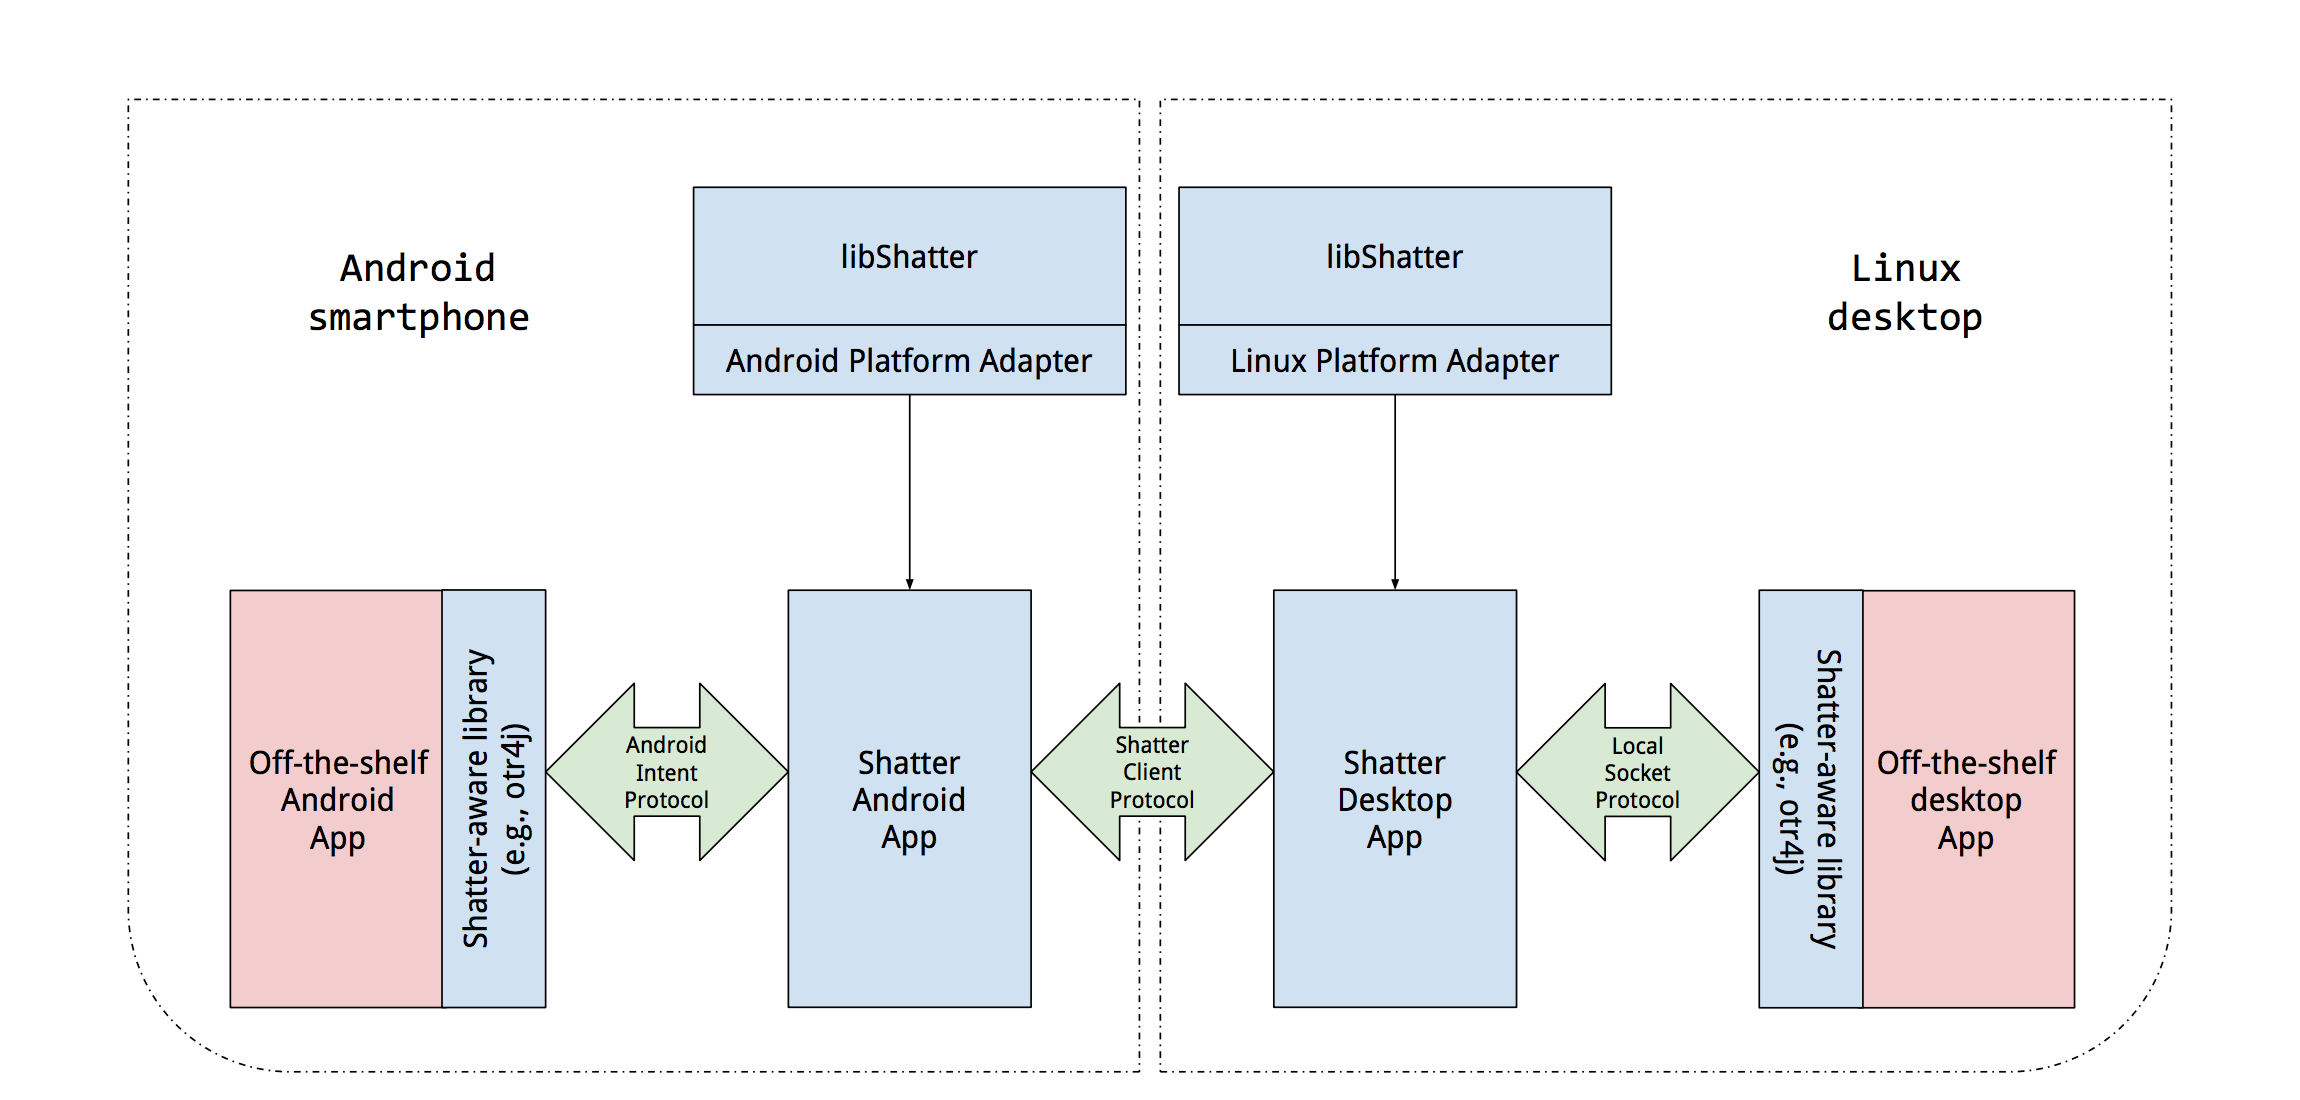
\includegraphics[width=\textwidth]{shatter}
	\caption{
		High-level architecture of the Shatter library\cite{Atwater2016}. 
		Android Wear devices run a Shatter client similar to the Android 					
		implementation (left), while Windows and macOS machines use a similar
		setup to the Linux example (right).}
	\label{fig:shatter}
\end{figure*}

\begin{enumerate}[label=\arabic*., wide, labelwidth=!, labelindent=0pt]
	\item \textbf{Cryptographic Algorithms:} Shatter has implementations of two threshold algorithms. The first is a $(t,n)$-Threshold-DSA 						signature 	scheme proposed by Gennaro et al. \cite{Gennaro}. This was chosen as it provides the authentication in most OTR (Off-The-Record) 			protocol implementations for which the authors later intend to add threshold cryptography support. The second threshold algorithm 							implemented is the Damgaard-Jurik (t,n)-threshold version of Paillier's additively homomorphic encryption algorithm \cite{Damgard2000}. 					This was chosen because it 	provides the properties required of the encryption algorithm used as a component of the aforementioned signature 			algorithm.
	\item \textbf{libShatter:} This is the library that provides the actual implementations of the cryptography protocols as well as classes to aid 					network connections between clients. It is written in Java (targeting versions 1.7+) ensuring that is easily portable to all major desktop and 				laptop computer platforms. It also compiles to an Android app library so it can be used in Android apps. libShatter consists of the following four 			major components:
	\begin{itemize}
		\item \textbf{ThresholdAgent:} This is a daemon that performs the core cryptography operations as well as device management. The 							NetworkAgent (described below) delegates the work of managing network connections, incoming packets and any received or pending 						requests to this daemon.
		\item \textbf{NetworkAgent:} This daemon manages the connections to all the user's other devices. It is also responsible for managing all the 		network communication that takes place between them.
		\item \textbf{Platform Adapters:} This is a package that contains adapters for platform-specific operations. It includes a set of classes that 				help to manipulate and store persistent configuration information with a uniform interface on various platforms.
		\item \textbf{Crypto:} This is a package containing the actual implementations of cryptographic protocols. It does not contain the network 				protocols, which are instead managed by ThresholdAgent These implementations are called by ThresholdAgent in order to perform threshold 				DSA 	operations. It also contains 	some convenience utilities, such as a class for generating cryptographically secure random numbers.
	\end{itemize}
	\item \textbf{Shatter desktop app:} This is the implementation for the Shatter desktop client application. It is implemented in Java as an 					interactive command-line application and allows making calls to ThresholdAgent, displaying and responding to requests and 											maintaining configurations. Developers can implement a UI with bindings to the various API functions.
	\item\textbf{Shatter Android app:} The Android app acts as the host service for the ThresholdAgent for all other apps on the device. This 					provides a central device management interface for users who may have multiple apps on which they wish to use thresholding installed on their 			phone.
	\item \textbf{Device Group management:} The user can connect any number of Shatter-compatible apps to a single instance of a Shatter client 			application. Thus, the user has the ability of managing multiple apps and devices from one place. The client takes care of new group formation, 			new device enrolment and old/lost device revocation. For formation of a new group, the user must initiate secure pairing either by scanning a QR 		code, or by verifying a displayed code on both screens. For enrolment and revocation, the user must gather a threshold number of devices 					together. The request is initiated on one device and then passed along to others in the group. The user must accept these requests on each 				device. This causes them to send their shares to the initiating device which can use these to regenerate the original private key. This is then used 		to generate a new set of shares (with/without the target device).
\end{enumerate}
	
%shatter applied to two apps: names and concluding remarks
The authors have demonstrated the feasibility of their work by implementing Shatter versions of two popular android apps, namely ChatSecure and OmniNotes. ChatSecure is an application offering the OTR (off- the-record messaging) protocol. The authors have modified the signing process in ChatSecure to use Shatter app's distributed DSA signature. OmniNotes is a simple note-taking application for Android. I offers very basic encryption for notes. The authors has improved the encryption by generating strong random keys and protecting them with a threshold encryption scheme.

Shatter is a free and open-source library and a good option for developers looking to add threshold cryptographic protections to their desktop and Android applications. Hopefully, future versions of the library will support more smartphone operating systems as well as extend support to IoT devices.

 

\subsection{Blockchains and Collective Signing}
Kokoris-Kogias et al.\cite{Kokoris-kogias} have developed a unique solution using blockchains and collective signing for SSH-key management. The system, in its current state, can only be used for SSH-key management but the authors are looking to expand this research to make a system that provides holistic identity management.

As it were, their system combines the ideas of a personal PKI and thresholding to solve the issue of key management as well as several accompanying issues such revocation of keys, loss/removal or addition of new devices and key storage. The authors have combined blockchains and collective signing to develop a secure and decentralized SSH-key management system. A cothority\cite{Syta} is used for SSH management and maintains a list of keys of the user.

\begin{figure}[h]
			\centering
			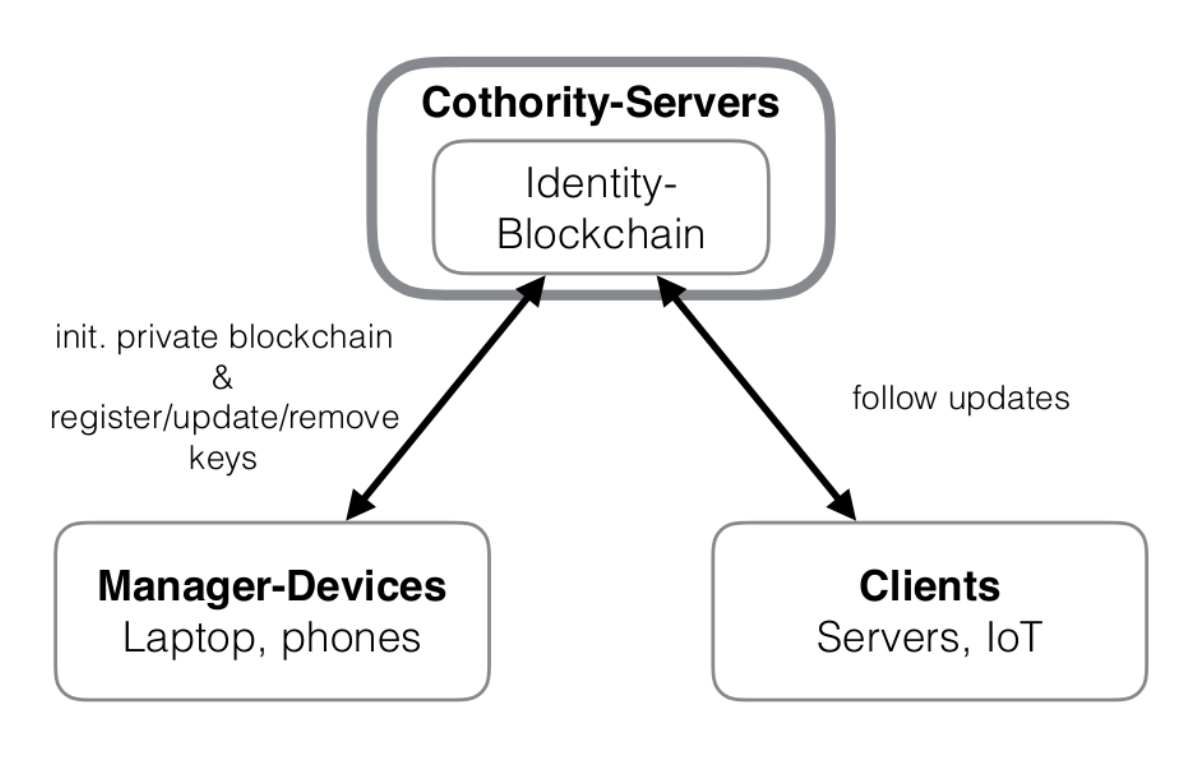
\includegraphics[width=\columnwidth]{cothority}
			\caption{Cothority server, devices and clients \cite{Kokoris-kogias}}
			\label{fig:cotho}
		\end{figure}
		
The \textit{cothority} is a group of publicly available servers that provide a blockchain management service. This resembles the notion of a personal PKI. The \textit{manager-devices} are devices that the user has physical access to such a laptops and mobile phones. They are instrumental to making changes and managing the user's identity but cannot manage the distributed co-ordination themselves which is why the cothority servers are required. Whenever users needs to add, remove or rotate keys they create an update-request and the cothority contacts  threshold number of manager devices. If this threshold number of devices agree on the change then the cothority updates the keys and models a forward link, making the blockchain doubly-linked. This process is fundamentally thresholding where a threshold number of devices must agree and sign. Lastly, the \textit{clients} are servers, IoT devices and services (e.g. GitHub) that users want to access. The clients download and verify the blocks from the cothority to update their access lists and are immediately notified of changes if they are online. Otherwise, they randomly poll the cothority when the come online and update their access lists.

The \textit{Identity-Blockchain} forms the basic structure of the system. It is composed of blocks that store the SSH-keys of the user's devices. These blocks are doubly-linked. The backward links are cryptographic hashes of the previous block. Future blocks do not exist at the time of creation of a block and thus cannot be incorporated in the current block's cryptographic hash. They are added inside the block later when a future block is created. When the cothority creates a new block and a threshold of managers sign it, a forward link is created from the current block to the new block and the new block is now made head of the chain. A client can easily follow this chain and verify the changes that have taken place because the threshold of devices use their current key to sign a new key and in the process delegate trust from the current key to the new key.

The authors plan to develop a larger Identity Management System that can be used to manage not only SSH-keys but also PGP keys and even keys for end-to-end encryption in instant messaging services so that users do not have to trust the operator of the service with their private keys. The system will be implemented based on CONIKS and use all of its privacy features such as hashed keys so a client can retrieve a block only through knowledge of the keys), symmetric-key encrypted userID (if the user does not want to be publicly reachable), etc. In addition, the system will user cothority servers, blockchains and collective signing. All in all, this is a novel approach to the multi-device problem and looks like a promising and emerging technology.


\section{Conclusion}

The field of multiple device and key management is a turbulent one with new ideas and methods constantly cropping up. The dust is yet to settle but when it does, it seems that some form of threshold cryptosystem will be the way forward. The idea of the personal PKI has held its own for over a decade and continues to be investigated while the idea of using threshold cryptography is in vogue as it solves many of the issues posed when implementing the former. If one would like to implement multiple device and key management one should try both options and evaluate them. The personal PKI systems work well if one is sure that there are low chances of one's device being lost or stolen. Contrariwise, one may wish to invest in threshold cryptosystems if devices are frequently lost or stolen or even rotated, removed and replaced. If one possess shared devices then \textit{webinos} is a good option as it does not equate device authentication with user authentication. Finally, if one simply possesses just two devices, then there is not much to be gained from going down the threshold cryptosystem route.

Ultimately, there is no clear winner and users must assess their situation and try the various options for themselves.

